% Provenance (never printed): old premiere S material on the structure of the
% Earth from seismology (P and S waves, travel times, the Moho, the shadow zone
% and the core, a reference model); see sources/book2/PROVENANCE.md. Profiles
% from figdata/grade-11/prem_profiles.py, rays and travel times from
% seismic_rays.py, the refraction lines and the problem's readings from
% moho_refraction.py. Lehmann's story and portrait are told in Book 1 (g6
% inside-the-earth): recalled here, not repeated.
\chapter{Gelombang Seismik Menyingkap Bagian Dalam Bumi}\label{ch:g11:seismic-structure}

Pada 8 Oktober 1909 sebuah gempa bumi mengguncang lembah Sungai Kupa, sekitar
\qty{40}{km} di tenggara Zagreb, di Kroasia. Beberapa bulan sebelumnya, Andrija
Mohorovičić telah memasang seismograf baru di Observatorium Meteorologi
Zagreb, dan alat itu merekam seluruh peristiwa itu. Ia lalu meminta rekaman
dari observatorium-observatorium lain dan mengumpulkan rekaman 41 stasiun. Pada
rekaman stasiun-stasiun yang lebih jauh ia menemukan sesuatu yang tidak
terduga: dua \omterm{def:g11:seismic-structure:body-waves}{gelombang P} yang terpisah, yang satu lemah lalu yang lain lebih
kuat, padahal seharusnya hanya ada satu. Dari pasangan gelombang itu ia
menyimpulkan bahwa batuan di bawah kerak berbeda, dan ia mengukur kedalaman
batasnya. Bab ini menunjukkan bagaimana waktu tiba gelombang gempa bumi
menyingkap lapisan-lapisan Bumi: dasar kerak, inti dan bagian luarnya yang cair,
dan seluruh bagian dalam Bumi, kedalaman demi kedalaman.
% ledger: herak:kupa-1909, srl:mohorovicic, geotech:moho-1909, kayal:pn-sn

\begin{recall}
Gempa bumi bermula di suatu titik di dalam Bumi, hiposentrum; titik di
permukaan tepat di atasnya adalah episentrum. Seismometer merekam guncangan
tanah, dan magnitudo mengukur besarnya gempa bumi (Buku 1, kelas 7). Bumi
mempunyai kerak, mantel, dan inti; inti mempunyai bagian luar yang cair dan
bagian dalam yang padat. Gelombang gempa bumi terutama ada dua jenis,
\omterm{def:g11:seismic-structure:body-waves}{gelombang P} yang lebih cepat dan \omterm{def:g11:seismic-structure:body-waves}{gelombang S} yang lebih lambat, dan \omterm{def:g11:seismic-structure:body-waves}{gelombang S}
tidak dapat menyeberangi zat cair (Buku 1, kelas 6). Gelombang yang
menyeberangi batas antara dua bahan, yang di dalamnya ia merambat dengan
kecepatan $v_1$ dan $v_2$, dibiaskan:
$\sin i_1/v_1 = \sin i_2/v_2$, dengan sudut diukur dari garis yang tegak lurus
pada batas itu (hukum Snell; buku-buku fisika).
\end{recall}

\section{Gelombang seismik dan waktu tempuh}

\subsection{Dua jenis gelombang badan}

Gempa bumi memancarkan gelombang ke segala arah. Sebagian merambat di sepanjang
permukaan; yang lain, gelombang badan, merambat melalui bagian dalam Bumi, dan
gelombang-gelombang inilah yang menyingkapnya.

\begin{definition}[Gelombang P; gelombang S]\label{def:g11:seismic-structure:body-waves}
Yang disebut \emph{gelombang P}\index{gelombang P} adalah gelombang seismik yang
secara bergantian memampatkan dan meregangkan batuan: batuan bergerak maju-mundur
searah dengan arah rambat gelombang itu. Gelombang ini menyeberangi zat padat,
zat cair, dan gas, dan merupakan gelombang seismik yang paling cepat, sehingga
tiba paling dahulu. Yang disebut \emph{gelombang S}\index{gelombang S} adalah
gelombang yang menggeser batuan: batuan bergerak tegak lurus pada arah rambat
gelombang itu. Gelombang ini hanya menyeberangi zat padat, dan tiba sesudah
gelombang P.
\end{definition}
% ledger: kayal:p-s

Zat cair mengalir dan tidak melawan perubahan bentuk, sehingga tidak dapat
meneruskan geseran: itulah sebabnya \omterm{def:g11:seismic-structure:body-waves}{gelombang S} berhenti di permukaan zat cair.
Pada kebanyakan batuan, \omterm{def:g11:seismic-structure:body-waves}{gelombang P} merambat sekitar $\sqrt 3 \approx 1.7$ kali
lebih cepat daripada \omterm{def:g11:seismic-structure:body-waves}{gelombang S}. Di kerak bagian atas, \omterm{def:g11:seismic-structure:body-waves}{gelombang P} merambat
dengan kecepatan sekitar \qty{5.8}{km/s} dan \omterm{def:g11:seismic-structure:body-waves}{gelombang S} sekitar
\qty{3.2}{km/s}; tepat di bawah kerak keduanya mencapai sekitar
\qty{8.1}{km/s} dan \qty{4.5}{km/s}.
% ledger: kayal:p-s, kayal:outer-core-liquid, data:prem (vp_surface 5.8, vs_surface 3.2,
% vp_upper_mantle 8.11, vs_upper_mantle 4.49 in figdata/grade-11/prem_profiles.py)

\begin{omfigure}
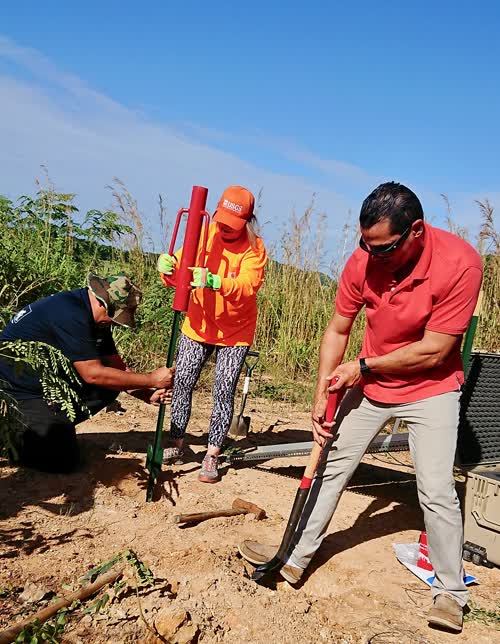
\includegraphics[width=0.5\linewidth]{images/book2/g11-usgs-seismometer.jpg}

{\small Para ahli seismologi dari Jaringan Seismik Puerto Riko dan dari USGS
memasang seismometer sementara di barat daya Puerto Riko, pada 10 Januari
2020. Foto: Thomas Pratt, USGS (domain publik).}
\end{omfigure}
% ledger: photo:g11-seismometer

\subsection{Kurva waktu tempuh}

Jarak dari gempa bumi ke stasiun yang jauh diukur sebagai sudut: sudut $\Delta$
di pusat Bumi di antara episentrum dan stasiun itu, yang disebut \emph{jarak
episentral}\index{jarak episentral}. Satu derajatnya sama dengan
$\qty{111.2}{km}$ di sepanjang permukaan.
% ledger: earth:Rmean

\begin{definition}[Waktu tempuh; kurva waktu tempuh]\label{def:g11:seismic-structure:travel-time}
Yang disebut \emph{waktu tempuh}\index{waktu tempuh} gelombang seismik di suatu
stasiun adalah waktu yang diperlukannya untuk merambat dari hiposentrum ke
stasiun itu. Yang disebut \emph{kurva waktu tempuh}\index{kurva waktu tempuh}
suatu gelombang adalah grafik waktu tempuhnya terhadap jarak episentral stasiun.
\end{definition}

Stasiun mencatat waktu tiba setiap gelombang; bila waktu terjadinya gempa bumi
diketahui, selisihnya adalah \omterm{def:g11:seismic-structure:travel-time}{waktu tempuh}. Ribuan gempa bumi yang direkam oleh
ribuan stasiun telah memberikan \omterm{def:g11:seismic-structure:travel-time}{kurva waktu tempuh} dengan sangat teliti. Pada
gambar, kurva-kurva itu dihitung dari \omterm{def:g11:seismic-structure:reference-model}{model acuan Bumi} pada
\cref{sec:g11:seismic-structure:model}, dan titik-titiknya adalah \omterm{def:g11:seismic-structure:travel-time}{waktu tempuh}
yang teramati pada gempa bumi yang nyata: keduanya sesuai sampai dua persen di
mana-mana, dan paling sering sampai satu atau dua detik.

\begin{omfigure}
\begin{tikzpicture}
\begin{axis}[omrecord, width=0.84\linewidth, height=6.4cm, xmin=0, xmax=180, ymin=0, ymax=30,
  xtick={0,20,...,180}, ytick={0,5,...,30},
  xlabel={jarak episentral $\Delta$ (derajat)}, ylabel={waktu tempuh (menit)},
  tick label style={font=\small}, label style={font=\small}, clip=false]
% computed in figdata/grade-11/seismic_rays.py; ledger: data:prem, auspass:surftim
\addplot[omDef, line width=0.9pt] table[x=delta_deg, y=t_min] {figdata/out/grade-11-seismic_rays-ttp.dat};
\addplot[omProp, line width=0.9pt] table[x=delta_deg, y=t_min] {figdata/out/grade-11-seismic_rays-tts.dat};
\addplot[omDef, line width=0.9pt, densely dashed] table[x=delta_deg, y=t_min] {figdata/out/grade-11-seismic_rays-ttpkp.dat};
\addplot[omDef!55, line width=0.9pt, densely dotted] table[x=delta_deg, y=t_min] {figdata/out/grade-11-seismic_rays-ttpkikp.dat};
\addplot[only marks, mark=*, mark size=1.5pt, black] table[x=delta_deg, y=p_min] {figdata/out/grade-11-seismic_rays-observed.dat};
\addplot[only marks, mark=*, mark size=1.5pt, black, unbounded coords=discard] table[x=delta_deg, y=s_min] {figdata/out/grade-11-seismic_rays-observed.dat};
\node[font=\small, text=omProp, anchor=south east] at (axis cs:68,21.2) {S};
\node[font=\small, text=omDef, anchor=north west] at (axis cs:72,11.2) {P};
\node[font=\small, text=omDef, anchor=south, align=center] at (axis cs:158,23.2) {P melalui\\inti};
\fill[black!10] (axis cs:98.5,0) rectangle (axis cs:143.8,3.2);
\node[font=\scriptsize, align=center] at (axis cs:121.1,1.6) {tanpa P langsung};
\end{axis}
\end{tikzpicture}

{\small \omterm{def:g11:seismic-structure:travel-time}{Kurva waktu tempuh} \omterm{def:g11:seismic-structure:body-waves}{gelombang P} (biru) dan \omterm{def:g11:seismic-structure:body-waves}{gelombang S} (jingga) dari
gempa bumi di permukaan, yang dihitung dengan \omterm{def:g11:seismic-structure:reference-model}{model acuan Bumi}; kurva putus-putus
dan bertitik adalah \omterm{def:g11:seismic-structure:body-waves}{gelombang P} yang telah menyeberangi inti (bertitik: inti
dalam). Titik hitam: \omterm{def:g11:seismic-structure:travel-time}{waktu tempuh} yang teramati. Di antara sekitar \ang{99} dan
\ang{144} tidak ada \omterm{def:g11:seismic-structure:body-waves}{gelombang P} yang tiba secara langsung (diarsir).}
\end{omfigure}

Kurva S naik lebih curam daripada kurva P, sehingga selang antara kedua kedatangan
itu bertambah seiring jarak. Hal ini memberikan jarak gempa bumi dari satu
rekaman saja.

\begin{method}[Jarak gempa bumi dari selang S--P]\label{met:g11:seismic-structure:distance}
\begin{enumerate}
  \item Pada rekaman, baca waktu \omterm{def:g11:seismic-structure:body-waves}{gelombang P} pertama dan \omterm{def:g11:seismic-structure:body-waves}{gelombang S}
        pertama; selisih keduanya adalah selang S--P.
  \item Pada \omterm{def:g11:seismic-structure:travel-time}{kurva waktu tempuh} (atau dalam tabelnya), cari jarak
        episentral tempat kurva S terletak sebesar selang itu di atas
        kurva P.
  \item Ubah ke kilometer, jika perlu, dengan $\qty{111.2}{km}$ per derajat.
\end{enumerate}
Dengan tiga stasiun, episentrum adalah titik yang berjarak tepat dari
ketiganya.
\end{method}

\begin{example}[Gempa bumi yang berjarak \ang{60}]\label{ex:g11:seismic-structure:sp}
\omterm{def:g11:seismic-structure:travel-time}{Waktu tempuh} yang teramati adalah \qty{608}{s} untuk P dan \qty{1101}{s} untuk S
pada \ang{60}, \qty{536}{s} dan \qty{967}{s} pada \ang{50}. Karena itu stasiun
yang merekam \omterm{def:g11:seismic-structure:body-waves}{gelombang S} \qty{493}{s} (8~menit 13~detik) sesudah \omterm{def:g11:seismic-structure:body-waves}{gelombang P}
terletak \ang{60} dari episentrum: sekitar $60 \times 111.2 \approx
\qty{6670}{km}$. Pada \ang{50} selangnya hanya \qty{431}{s}.
\end{example}
% ledger: auspass:surftim

\begin{omfigure}
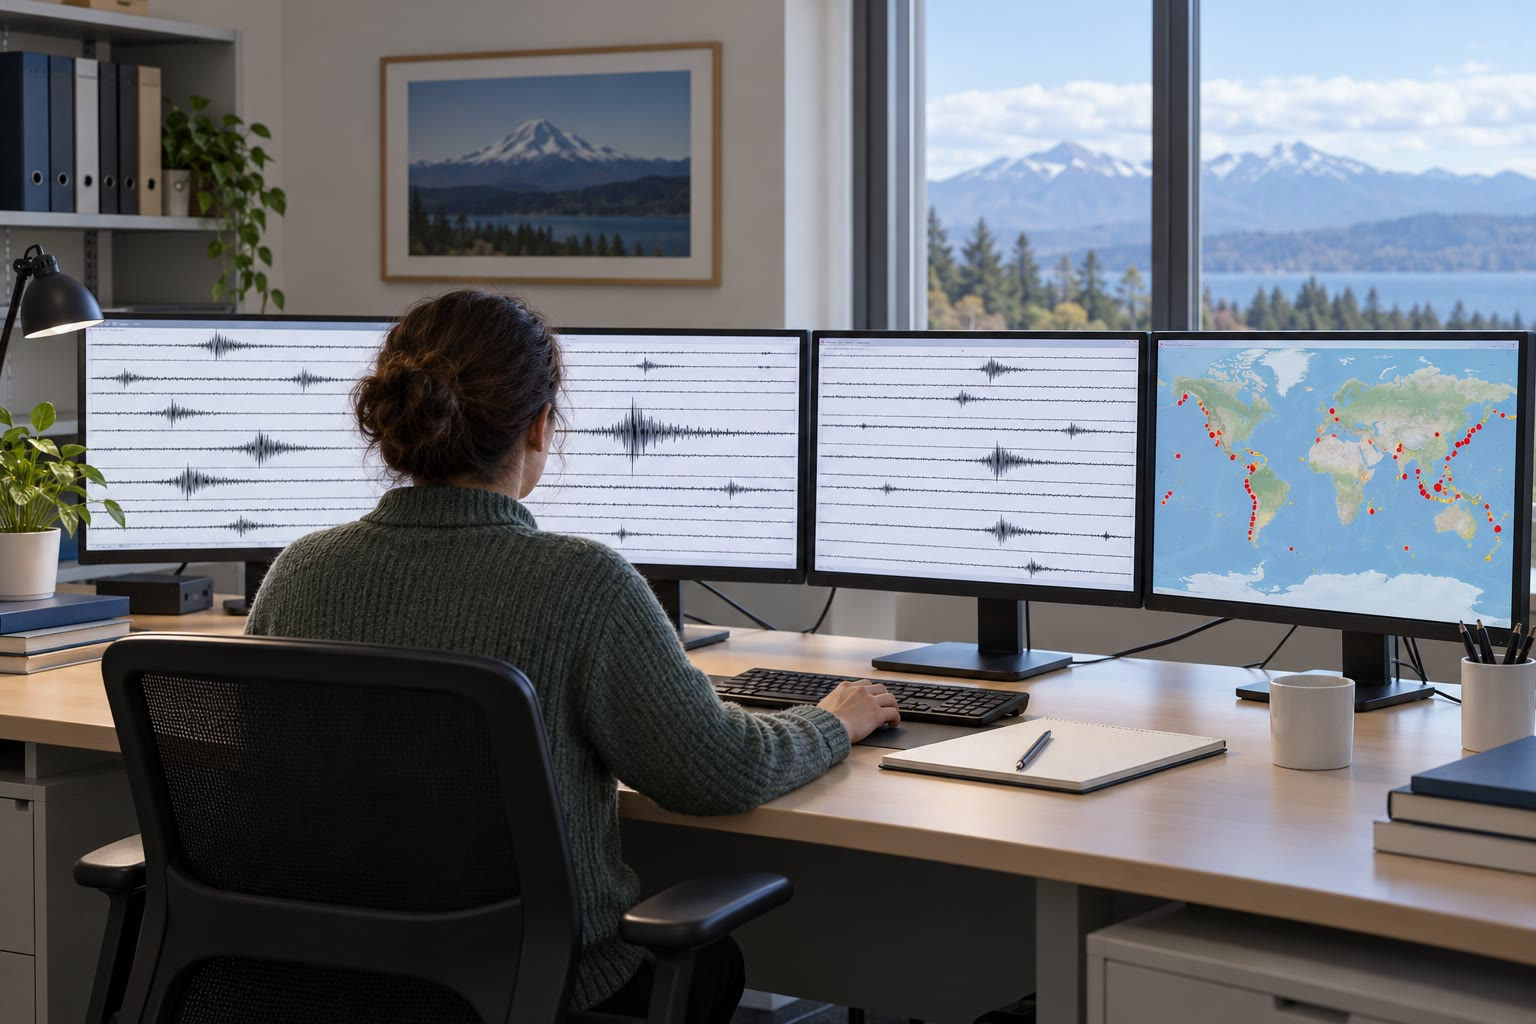
\includegraphics[width=0.66\linewidth]{images/book2/ai/g11-seismology-observatory.jpg}

{\small Di sebuah observatorium seismologi, rekaman banyak stasiun ditampilkan
berdampingan, dan gempa bumi yang ditentukan letaknya oleh rekaman itu
digambarkan pada peta dunia (ilustrasi AI).}
\end{omfigure}

\section{Pembiasan dan Moho}\label{sec:g11:seismic-structure:moho}

\subsection{Gelombang yang merambat di sepanjang batas}

Di dalam Bumi kecepatan gelombang seismik berubah seiring kedalaman, sebagian
besar secara berangsur, tetapi di beberapa tempat secara mendadak.

\begin{definition}[Diskontinuitas seismik]\label{def:g11:seismic-structure:discontinuity}
Yang disebut \emph{diskontinuitas seismik}\index{diskontinuitas seismik} adalah
permukaan di dalam Bumi yang padanya kecepatan gelombang seismik berubah secara
mendadak --- dalam ketebalan yang jauh lebih kecil daripada panjang gelombangnya.
\end{definition}

Pada diskontinuitas, sebagian gelombang dipantulkan dan sebagian dibiaskan.
Ambillah lapisan setebal $h$ yang di dalamnya \omterm{def:g11:seismic-structure:body-waves}{gelombang P} merambat dengan
kecepatan $v_1$, di atas lapisan yang di dalamnya gelombang itu lebih cepat,
$v_2 > v_1$. Sinar yang turun dengan sudut $i$ dari garis vertikal dibiaskan
dengan sudut $r$ yang diberikan oleh $\sin r = (v_2/v_1)\sin
i$: sinar itu dibelokkan menjauhi garis vertikal. Ketika $\sin i$ mencapai
$v_1/v_2$, sinar bias merambat tepat di sepanjang batas. Sudut
\[
  i_c, \qquad \sin i_c = \frac{v_1}{v_2},
\]
disebut \emph{sudut kritis}\index{sudut kritis}. Gelombang yang dibiaskan pada
\omterm{ex:g11:seismic-structure:sp}{sudut kritis} merambat di sepanjang bagian atas lapisan yang lebih cepat dengan
kecepatan $v_2$, dan sambil merambat ia memancarkan gelombang kembali ke atas ke
lapisan atas, semuanya dengan sudut $i_c$: gelombang-gelombang itu mencapai
permukaan sebagai \emph{gelombang kepala}\index{gelombang kepala}.

\begin{omfigure}
\begin{tikzpicture}[x=0.05cm, y=0.05cm, font=\footnotesize, >={Stealth[length=4pt]}]
% geometry from figdata/grade-11/moho_refraction.py: v1 6.2, v2 8.1, h 30 km, ic 49.9 deg
  \fill[omLithGranite!45] (-10,0) rectangle (215,-30);
  \fill[omLithPeridotite!45] (-10,-30) rectangle (215,-48);
  \draw[line width=0.6pt] (-10,0) -- (215,0);
  \draw[line width=0.9pt] (-10,-30) -- (215,-30);
  \node[anchor=west, align=left] at (218,-15) {kerak\\$v_1 = \qty{6.2}{km/s}$};
  \node[anchor=west, align=left] at (218,-39) {mantel\\$v_2 = \qty{8.1}{km/s}$};
  \node[anchor=east] at (215,-26) {Moho};
  % source and station
  \fill[omDef] (0,0) circle (1.6);
  \node[anchor=south] at (0,1.5) {gempa bumi};
  \draw[fill=white] (197,0) -- (203,0) -- (200,5) -- cycle;
  \node[anchor=south] at (200,5) {stasiun};
  % direct wave
  \draw[->, omProp, line width=0.8pt] (2,-2) -- (196,-2);
  \node[anchor=south, text=omProp] at (100,0.3) {gelombang langsung, kecepatan $v_1$};
  % head wave
  \draw[omDef, line width=0.9pt] (0,0) -- (35.7,-30);
  \draw[->, omDef, line width=0.9pt] (35.7,-30) -- (100,-30);
  \draw[omDef, line width=0.9pt] (100,-30) -- (164.3,-30) -- (200,0);
  \node[anchor=north, text=omDef] at (100,-31) {di sepanjang Moho dengan $v_2$};
  \foreach \x in {50,70,90,110,130,150} {
    \draw[->, omDef!60, densely dashed] (\x,-30) -- ++(25.5,21.5);
  }
  % critical angle
  \draw[black!60, densely dotted] (35.7,-30) -- (35.7,-8);
  \draw[black!70] (35.7,-18) arc[start angle=90, end angle=130.05, radius=12];
  \node[anchor=south east] at (33,-16) {$i_c$};
  % thickness and critical distance
  \draw[<->] (-6,0) -- (-6,-30);
  \node[anchor=east] at (-7,-15) {$h$};
\end{tikzpicture}

{\small Gelombang langsung dan \omterm{ex:g11:seismic-structure:sp}{gelombang kepala} (dengan skala sebenarnya: kerak
setebal \qty{30}{km}). \omterm{ex:g11:seismic-structure:sp}{Gelombang kepala} turun dengan \omterm{ex:g11:seismic-structure:sp}{sudut kritis} $i_c$,
merambat di sepanjang bagian atas mantel dan naik kembali dengan sudut $i_c$;
di sepanjang seluruh lintasannya di \omterm{def:g11:seismic-structure:moho}{Moho} ia memancarkan gelombang ke atas ke
permukaan (putus-putus). Gelombang itu tidak mencapai stasiun yang lebih dekat
daripada $2h\tan i_c$, sekitar \qty{71}{km} di sini.}
\end{omfigure}

\begin{proposition}[Waktu tempuh gelombang kepala]\label{prop:g11:seismic-structure:head-wave}
Untuk sumber di permukaan, stasiun pada jarak $x \ge 2h\tan i_c$
menerima \omterm{ex:g11:seismic-structure:sp}{gelombang kepala} sesudah
\[
  t(x) = \frac{x}{v_2} + \frac{2h\cos i_c}{v_1}.
\]
\omterm{def:g11:seismic-structure:travel-time}{Kurva waktu tempuhnya} adalah garis lurus dengan kemiringan $1/v_2$ yang, bila
diperpanjang ke belakang, memotong sumbu waktu pada \emph{waktu
intersep}\index{waktu intersep} $t_i = 2h\cos i_c/v_1$.
\end{proposition}

\begin{proof}
Sinar itu turun menempuh kaki miring sepanjang $h/\cos i_c$, yang maju secara
mendatar sejauh $h\tan i_c$; hal yang sama terjadi ketika naik. Di antaranya
sinar itu merambat di sepanjang batas sejauh $x - 2h\tan i_c$. Waktunya adalah
\[
  t = \frac{2h}{v_1\cos i_c} + \frac{x - 2h\tan i_c}{v_2}
    = \frac{x}{v_2} + \frac{2h}{v_1\cos i_c} - \frac{2h\sin i_c}{v_2\cos i_c}.
\]
Karena $1/v_2 = \sin i_c/v_1$, dua suku terakhir menjadi
$\frac{2h}{v_1\cos i_c}\,(1 - \sin^2 i_c) = \frac{2h\cos i_c}{v_1}$.
\end{proof}

Gelombang langsung tiba sesudah $x/v_1$: kurvanya adalah garis yang melalui
titik asal, lebih curam daripada garis \omterm{ex:g11:seismic-structure:sp}{gelombang kepala}. Di dekat sumber
gelombang langsung tiba lebih dahulu; jauh dari sumber, \omterm{ex:g11:seismic-structure:sp}{gelombang kepala}, yang
telah menempuh sebagian besar jalannya dengan kecepatan yang lebih tinggi,
menyusulnya.

\begin{proposition}[Jarak silang]\label{prop:g11:seismic-structure:crossover}
\omterm{ex:g11:seismic-structure:sp}{Gelombang kepala} tiba sebelum gelombang langsung di luar \emph{jarak
silang}\index{jarak silang}
\[
  x_c = 2h\sqrt{\frac{v_2 + v_1}{v_2 - v_1}}.
\]
\end{proposition}

\begin{proof}
Keduanya tiba bersamaan ketika $x/v_1 = x/v_2 + 2h\cos i_c/v_1$, yaitu
$x\,(v_2 - v_1)/(v_1 v_2) = 2h\cos i_c/v_1$, jadi $x = 2h\cos i_c\,v_2/(v_2 -
v_1)$. Padahal $\cos i_c = \sqrt{1 - v_1^2/v_2^2} = \sqrt{(v_2 - v_1)(v_2 +
v_1)}/v_2$, sehingga $x = 2h\sqrt{(v_2 + v_1)(v_2 - v_1)}/(v_2 - v_1) =
2h\sqrt{(v_2 + v_1)/(v_2 - v_1)}$. Di luar jarak itu \omterm{ex:g11:seismic-structure:sp}{gelombang kepala}, yang
garisnya kurang curam, tiba lebih dahulu.
\end{proof}

\begin{omfigure}
\begin{tikzpicture}
\begin{axis}[omrecord, width=0.78\linewidth, height=5.6cm, xmin=0, xmax=300, ymin=0, ymax=50,
  xtick={0,50,...,300}, xlabel={jarak dari episentrum (\unit{km})}, ylabel={waktu tempuh (\unit{s})},
  tick label style={font=\small}, label style={font=\small}, clip=false]
% computed in figdata/grade-11/moho_refraction.py (critical_km 71.4, crossover_km 164.6, intercept_s 6.23)
\addplot[omProp, line width=0.9pt] table[x=x, y=tdirect] {figdata/out/grade-11-moho_refraction-model.dat};
\addplot[omDef, line width=0.9pt, restrict x to domain=71:300] table[x=x, y=thead] {figdata/out/grade-11-moho_refraction-model.dat};
\addplot[omDef, densely dashed, restrict x to domain=0:72] table[x=x, y=thead] {figdata/out/grade-11-moho_refraction-model.dat};
\draw[black!50, densely dotted] (axis cs:164.6,0) -- (axis cs:164.6,26.5);
\node[font=\scriptsize, anchor=north] at (axis cs:164.6,0) {$x_c$};
\fill (axis cs:0,6.23) circle (1.5pt);
\draw[black!60] (axis cs:0.8,6.6) -- (axis cs:6,12);
\node[font=\scriptsize, anchor=south west, inner sep=1pt] at (axis cs:5,12) {$t_i = \qty{6.2}{s}$};
\node[font=\small, text=omProp, anchor=south east] at (axis cs:250,41) {gelombang langsung};
\node[font=\small, text=omDef, anchor=north west] at (axis cs:235,33) {gelombang kepala};
\end{axis}
\end{tikzpicture}

{\small \omterm{def:g11:seismic-structure:travel-time}{Waktu tempuh} gelombang langsung dan \omterm{ex:g11:seismic-structure:sp}{gelombang kepala} untuk kerak pada
gambar sebelumnya. Garis \omterm{ex:g11:seismic-structure:sp}{gelombang kepala}, bila diperpanjang ke belakang
(putus-putus), memotong sumbu waktu pada \omterm{prop:g11:seismic-structure:head-wave}{waktu intersep}; di luar \omterm{prop:g11:seismic-structure:crossover}{jarak silang}
$x_c \approx
\qty{165}{km}$ \omterm{ex:g11:seismic-structure:sp}{gelombang kepala} tiba lebih dahulu.}
\end{omfigure}

\subsection{Dasar kerak}

\begin{definition}[Moho]\label{def:g11:seismic-structure:moho}
Yang disebut \emph{diskontinuitas Mohorovičić}\index{diskontinuitas Mohorovičić},
atau \emph{Moho}\index{Moho}, adalah \omterm{def:g11:seismic-structure:discontinuity}{diskontinuitas seismik} di dasar kerak,
tempat kecepatan \omterm{def:g11:seismic-structure:body-waves}{gelombang P} melonjak dari paling tinggi sekitar \qty{7}{km/s}
menjadi sekitar \qty{8}{km/s}, kecepatan di mantel paling atas.
\end{definition}
% ledger: kayal:pn-sn, data:prem (6.8 -> 8.11 at 24.4 km)

\begin{history}[Mohorovičić dan dua gelombang P, 1909]
Andrija Mohorovičić (1857--1936) menemukan, pada rekaman gempa bumi tahun
1909, bahwa di luar jarak tertentu --- umumnya antara 100 dan
\qty{150}{km} --- \omterm{def:g11:seismic-structure:body-waves}{gelombang P} yang lemah dan lebih cepat tiba sebelum \omterm{def:g11:seismic-structure:body-waves}{gelombang
P} yang kuat. Ia menjelaskannya sebagai gelombang yang telah merambat melalui
batuan yang lebih cepat di bawah kerak. Ia menamai kedua gelombang itu Pg
(gelombang langsung di kerak) dan Pn (\omterm{ex:g11:seismic-structure:sp}{gelombang kepala} di sepanjang bagian atas
mantel), melakukan hal yang sama untuk \omterm{def:g11:seismic-structure:body-waves}{gelombang S}, dan menyimpulkan kecepatan
kedua lapisan itu serta kedalaman batas di antara keduanya. Gelombang Pn
merambat dengan kecepatan sekitar \qty{8.0}{km/s}, kecepatan mantel paling
atas. Makalah-makalahnya tahun 1910 membuktikan bahwa kerak dan mantel
berbeda; batas itu menyandang namanya.
\end{history}
% ledger: kayal:pn-sn, srl:mohorovicic

\begin{method}[Kedalaman Moho dari diagram waktu tempuh]\label{met:g11:seismic-structure:moho}
\begin{enumerate}
  \item Gambarkan waktu tiba pertama terhadap jarak dari
        episentrum.
  \item Tarik garis gelombang langsung (melalui titik asal) dan garis
        \omterm{ex:g11:seismic-structure:sp}{gelombang kepala}; kemiringannya adalah $1/v_1$ dan $1/v_2$.
  \item Perpanjang garis \omterm{ex:g11:seismic-structure:sp}{gelombang kepala} ke belakang sampai sumbu waktu:
        garis itu memotongnya pada \omterm{prop:g11:seismic-structure:head-wave}{waktu intersep} $t_i$.
  \item Dengan $\sin i_c = v_1/v_2$, tebal kerak adalah
        $h = \dfrac{v_1\,t_i}{2\cos i_c}$.
\end{enumerate}
\end{method}

\begin{example}[Kerak setebal \qty{30}{km}]\label{ex:g11:seismic-structure:moho}
Dengan $v_1 = \qty{6.2}{km/s}$ dan $v_2 = \qty{8.1}{km/s}$, $\sin i_c = 0.765$,
$i_c \approx \ang{49.9}$, dan $\cos i_c \approx 0.644$. \omterm{prop:g11:seismic-structure:head-wave}{Waktu intersep}
\qty{6.23}{s} memberikan $h = 6.2 \times 6.23/(2 \times 0.644) \approx
\qty{30}{km}$. \omterm{ex:g11:seismic-structure:sp}{Gelombang kepala} pertama kali mencapai permukaan pada
$2h\tan i_c \approx \qty{71}{km}$ dan menyusul gelombang langsung di luar
$x_c = 60\sqrt{14.3/1.9} \approx \qty{165}{km}$.
\end{example}
% values computed in figdata/grade-11/moho_refraction.py (ic_deg 49.9, critical_km 71.4, crossover_km 164.6)

Bila diukur dengan cara ini di seluruh dunia, \omterm{def:g11:seismic-structure:moho}{Moho} hanya terletak sekitar
\qty{5}{km} di bawah dasar samudra. Di bawah benua, \omterm{def:g11:seismic-structure:moho}{Moho} terletak rata-rata
sekitar \qty{41}{km} di bawah permukaan: sekitar \qty{30}{km} di tempat kerak
telah teregang, lebih dari \qty{45}{km} di bawah sabuk pegunungan, dan sampai
sekitar \qty{100}{km} di bawah jajaran pegunungan yang paling tinggi. Kerak
adalah kulit yang tipis: bahkan \qty{41}{km} kurang dari satu persen jari-jari
Bumi.
% ledger: usgs:crust-thickness, cm95:crust, kayal:discontinuities

\section{Inti}

\subsection{Sinar yang melengkung}

Di mantel, kecepatan gelombang seismik bertambah seiring kedalaman. Sinar yang
turun menyeberangi batuan yang makin lama makin cepat dan, menurut hukum Snell,
pada setiap langkah dibelokkan sedikit lebih jauh dari garis vertikal:
lintasannya melengkung dan berbalik naik ke arah permukaan. Makin dalam sinar
berbalik, makin jauh dari gempa bumi ia naik kembali. Gambar ini menunjukkan
sinar-sinar seperti itu, yang dihitung dengan kecepatan \omterm{def:g11:seismic-structure:reference-model}{model acuan Bumi}.

\begin{omfigure}
\begin{tikzpicture}
\begin{axis}[width=0.66\linewidth, height=0.66\linewidth, axis equal image, hide axis,
  xmin=-1.18, xmax=1.18, ymin=-1.18, ymax=1.2, clip=false]
% computed in figdata/grade-11/seismic_rays.py; ledger: data:prem
\fill[omLithPeridotite!25] (axis cs:0,0) circle [radius=1];
\fill[omSea!45] (axis cs:0,0) circle [radius=0.5462];
\fill[omSea!80] (axis cs:0,0) circle [radius=0.1917];
\addplot[black, line width=0.6pt, domain=0:360, samples=181] ({cos(x)}, {sin(x)});
\addplot[black!60, line width=0.4pt, domain=0:360, samples=181] ({0.5462*cos(x)}, {0.5462*sin(x)});
\addplot[black!60, line width=0.4pt, domain=0:360, samples=91] ({0.1917*cos(x)}, {0.1917*sin(x)});
\addplot[omDef, line width=0.6pt] table {figdata/out/grade-11-seismic_rays-praysmantle.dat};
\addplot[omDef!70!black, line width=0.6pt] table {figdata/out/grade-11-seismic_rays-prayscore.dat};
\addplot[omProp, line width=0.6pt] table {figdata/out/grade-11-seismic_rays-srays.dat};
% P shadow zone: 98.5 to 143.8 degrees from the source (right); S beyond 102.7 (left)
\addplot[black!80, line width=3pt, domain=-53.8:-8.5, samples=40] ({1.04*cos(x)}, {1.04*sin(x)});
\addplot[omProp!60, line width=3pt, domain=192.7:270, samples=40] ({1.04*cos(x)}, {1.04*sin(x)});
\fill[omDef] (axis cs:0,1) circle (2pt);
\node[font=\footnotesize, anchor=south] at (axis cs:0,1.04) {gempa bumi};
\node[font=\footnotesize, anchor=west, align=left] at (axis cs:1.07,-0.42) {tanpa P langsung\\(\ang{99}--\ang{144})};
\node[font=\footnotesize, anchor=east, align=right] at (axis cs:-1.07,-0.62) {tanpa S langsung\\di luar \ang{103}};
\node[font=\footnotesize, text=omDef, anchor=south west] at (axis cs:0.55,0.8) {P};
\node[font=\footnotesize, text=omProp, anchor=south east] at (axis cs:-0.55,0.8) {S};
\node[font=\scriptsize] at (axis cs:-0.5,-0.62) {mantel};
\node[font=\scriptsize] at (axis cs:-0.3,0.2) {inti luar};
\draw[black!70] (axis cs:-0.1,-0.06) -- (axis cs:-0.26,-0.22);
\node[font=\scriptsize, anchor=north east, inner sep=1pt] at (axis cs:-0.24,-0.22) {inti dalam};
\end{axis}
\end{tikzpicture}

{\small Sinar dari gempa bumi di puncak Bumi, yang dihitung dengan kecepatan
model acuan. Kanan: sinar P yang berbalik di mantel, sampai sekitar \ang{99},
dan sinar P yang menyeberangi inti dan keluar di luar sekitar \ang{144}; di
antaranya, tidak ada sinar P yang tiba secara langsung. Kiri: sinar S, yang
berbalik di mantel; tidak ada yang menyeberangi inti luar yang cair, dan tidak
ada \omterm{def:g11:seismic-structure:body-waves}{gelombang S} langsung yang mencapai jarak di luar sekitar \ang{103}.}
\end{omfigure}

\subsection{Zona bayangan dan inti luar yang cair}

Pada tahun 1906, ahli seismologi Oldham memperhatikan bahwa \omterm{def:g11:seismic-structure:body-waves}{gelombang P} yang
direkam di sisi Bumi yang berseberangan dengan gempa bumi tiba terlambat
dibandingkan dengan waktu yang diharapkan, dan ia mengusulkan adanya inti
pusat yang di dalamnya gelombang itu merambat lebih lambat. Pada tahun 1912
Gutenberg menunjukkan bahwa \omterm{def:g11:seismic-structure:body-waves}{gelombang P} tidak mencapai satu pita jarak yang
utuh, antara sekitar \ang{105} dan \ang{143}, dengan kedatangan yang kuat tepat
di luar \ang{143}; pada tahun 1914 ia menempatkan puncak inti pada kedalaman
\qty{2900}{km}.
% ledger: kayal:discontinuities, kayal:shadow

\begin{definition}[Zona bayangan]\label{def:g11:seismic-structure:shadow-zone}
Yang disebut \emph{zona bayangan}\index{zona bayangan} suatu gelombang seismik
adalah rentang jarak episentral yang tidak dapat dicapai gelombang itu secara
langsung dari gempa bumi, karena inti membelokkannya atau menghentikannya.
\end{definition}

Sinar-sinar itu menjelaskannya. Sinar P yang berbalik tepat di atas inti naik
kembali sekitar \ang{100} dari gempa bumi. Sinar yang turun sedikit lebih curam
masuk ke inti, tempat kecepatan P turun mendadak dari \qty{13.7}{km/s} menjadi
sekitar \qty{8.1}{km/s}: menurut hukum Snell sinar itu dibelokkan \emph{mendekati}
garis vertikal, menyeberangi inti, dan muncul jauh lebih jauh, di luar sekitar
\ang{144}. Tidak ada sinar P yang berbalik di mantel dan tidak ada sinar P yang
menyeberangi inti yang jatuh di antaranya. Dalam model acuan, \omterm{def:g11:seismic-structure:shadow-zone}{zona bayangan} P
membentang dari \ang{98.5} sampai \ang{143.8}, dekat dengan \ang{105}--\ang{143}
milik Gutenberg.
% ledger: kayal:shadow, data:prem (vp_above_cmb 13.72, vp_below_cmb 8.06); computed in
% figdata/grade-11/seismic_rays.py (shadow_start_deg 98.5, shadow_end_pkp_deg 143.8)

\omterm{def:g11:seismic-structure:body-waves}{Gelombang S} memberi tahu lebih banyak. Tidak ada \omterm{def:g11:seismic-structure:body-waves}{gelombang S} yang menyeberangi
inti luar: inti luar tidak meneruskan gelombang geser, jadi inti luar itu cair.
Akibatnya, tidak ada \omterm{def:g11:seismic-structure:body-waves}{gelombang S} yang tiba secara langsung di luar sekitar
\ang{103} dalam model acuan --- di seluruh sisi Bumi yang berseberangan.
% ledger: kayal:outer-core-liquid; computed in figdata/grade-11/seismic_rays.py (s_direct_max_deg 102.7)

\begin{definition}[Batas inti--mantel; batas inti dalam]\label{def:g11:seismic-structure:core}
Yang disebut \emph{batas inti--mantel}\index{batas inti--mantel} adalah
\omterm{def:g11:seismic-structure:discontinuity}{diskontinuitas seismik} antara mantel yang padat dan inti luar yang cair, pada
kedalaman \qty{2891}{km}; di sana kecepatan P turun dari sekitar
\qty{13.7}{km/s} menjadi sekitar \qty{8.1}{km/s}, dan \omterm{def:g11:seismic-structure:body-waves}{gelombang S} berhenti.
Yang disebut \emph{batas inti dalam}\index{batas inti dalam}, pada kedalaman
\qty{5150}{km}, memisahkan inti luar yang cair dari inti dalam yang padat; di
sana kecepatan P melonjak dari sekitar \qty{10.4}{km/s} menjadi sekitar
\qty{11.0}{km/s}.
\end{definition}
% ledger: data:prem, prem:cmb, prem:icb (Book 3 rows); values in figdata/grade-11/prem_profiles.py

\omterm{def:g11:seismic-structure:shadow-zone}{Zona bayangan} tidak sepenuhnya sunyi: \omterm{def:g11:seismic-structure:body-waves}{gelombang P} yang lemah tiba di dalamnya.
Inge Lehmann menjelaskannya pada tahun 1936 dengan inti dalam yang padat, yang
di dalamnya \omterm{def:g11:seismic-structure:body-waves}{gelombang P} merambat lebih cepat (Buku 1, kelas 6). Sinar-sinar itu
menunjukkan caranya. Sinar P yang mencapai inti dalam dibelokkan menjauhi garis
vertikal di tempat kecepatannya melonjak, seperti di \omterm{def:g11:seismic-structure:moho}{Moho}, dan keluar dari inti
lebih cepat: dalam model acuan, sinar yang melalui inti dalam mencapai permukaan
mulai sekitar \ang{121}, di dalam \omterm{def:g11:seismic-structure:shadow-zone}{zona bayangan} (kurva bertitik pada gambar
\omterm{def:g11:seismic-structure:travel-time}{waktu tempuh}).
% ledger: nbi:lehmann-1936 (Book 1 row), kayal:lehmann; computed in
% figdata/grade-11/seismic_rays.py (pkikp_min_deg 121.4)

\section{Model acuan Bumi}\label{sec:g11:seismic-structure:model}

Bila digabungkan, jutaan \omterm{def:g11:seismic-structure:travel-time}{waktu tempuh} memberikan kecepatan \omterm{def:g11:seismic-structure:body-waves}{gelombang P} dan S
pada setiap kedalaman. Kecepatan itu bergantung pada batuan dan massa jenisnya,
dan massa total Bumi menentukan massa jenis rata-ratanya; bersama-sama keduanya
juga memberikan massa jenis pada setiap kedalaman.
% ledger: data:prem, prem:constraints (Book 3 row)

\begin{definition}[Model acuan Bumi]\label{def:g11:seismic-structure:reference-model}
Yang disebut \emph{model acuan Bumi}\index{model acuan Bumi} adalah tabel
kecepatan \omterm{def:g11:seismic-structure:body-waves}{gelombang P}, kecepatan \omterm{def:g11:seismic-structure:body-waves}{gelombang S}, dan massa jenis terhadap
kedalaman, yang sama ke segala arah, yang dipilih agar sesuai dengan \omterm{def:g11:seismic-structure:travel-time}{waktu
tempuh} gelombang seismik yang teramati dan dengan massa Bumi.
\end{definition}

Model yang paling banyak dipakai adalah Model Acuan Bumi Pendahuluan
(PREM, dari singkatan nama Inggrisnya), yang diterbitkan oleh A.~M.~Dziewonski dan D.~L.~Anderson pada tahun
1981. Sinar dan \omterm{def:g11:seismic-structure:travel-time}{waktu tempuh} dalam bab ini dihitung dengan model itu: \omterm{def:g11:seismic-structure:travel-time}{waktu
tempuh} P pada \ang{60}, misalnya, menjadi \qty{607}{s}, dibandingkan dengan
\qty{608}{s} yang teramati.
% ledger: data:prem, auspass:surftim; computed in figdata/grade-11/seismic_rays.py (p_60_s 607.2)

\begin{omfigure}
\begin{tikzpicture}
\begin{axis}[omrecord, width=0.86\linewidth, height=6.2cm, xmin=0, xmax=6371, ymin=0, ymax=14.5,
  xtick={0,1000,...,6000}, ytick={0,2,...,14}, scaled x ticks=false,
  xticklabel style={/pgf/number format/1000 sep={\,}},
  xlabel={kedalaman (\unit{km})}, ylabel={kecepatan (\unit{km/s}) atau massa jenis (\unit{g/cm^3})},
  tick label style={font=\small}, label style={font=\small}, clip=false]
% computed in figdata/grade-11/prem_profiles.py; ledger: data:prem
\addplot[omDef, line width=0.9pt] table[x=depth, y=vp] {figdata/out/grade-11-prem_profiles-profile.dat};
\addplot[omProp, line width=0.9pt] table[x=depth, y=vs] {figdata/out/grade-11-prem_profiles-profile.dat};
\addplot[black, line width=0.9pt, densely dashed] table[x=depth, y=rho] {figdata/out/grade-11-prem_profiles-profile.dat};
\foreach \d in {670,2891,5149.5} {\edef\temp{\noexpand\draw[black!40, densely dotted] (axis cs:\d,0) -- (axis cs:\d,14.5);}\temp}
\node[font=\scriptsize, anchor=south, align=center] at (axis cs:2891,14.5) {batas\\inti--mantel};
\node[font=\scriptsize, anchor=south, align=center] at (axis cs:5149.5,14.5) {batas\\inti dalam};
\node[font=\scriptsize, anchor=south] at (axis cs:670,14.5) {\qty{670}{km}};
\node[font=\small, text=omDef, anchor=south] at (axis cs:1800,12.4) {kecepatan P};
\node[font=\small, text=omProp, anchor=south] at (axis cs:1800,7.0) {kecepatan S};
\node[font=\small, anchor=north] at (axis cs:1800,4.5) {massa jenis};
\node[font=\scriptsize, align=center] at (axis cs:4000,1.9) {tanpa gelombang S:\\cair};
\end{axis}
\end{tikzpicture}

{\small Kecepatan \omterm{def:g11:seismic-structure:body-waves}{gelombang P} dan S serta massa jenis terhadap kedalaman dalam
Model Acuan Bumi Pendahuluan, PREM (Dziewonski dan Anderson, 1981). Garis-garis
bertitik menandai diskontinuitas utama di bawah \omterm{def:g11:seismic-structure:moho}{Moho}, yang terlalu dangkal
untuk tampak pada skala ini.}
\end{omfigure}

Membaca model itu dari atas:
\begin{itemize}
  \item kerak, dengan kecepatan P 5.8 sampai \qty{6.8}{km/s}, berakhir di \omterm{def:g11:seismic-structure:moho}{Moho}
        (\qty{24.4}{km} dalam model rata-rata ini);
  \item di mantel, kecepatan bertambah seiring kedalaman, dengan lompatan
        mendadak yang lebih kecil, yang terbesar di dekat \qty{400}{km} dan
        \qty{670}{km};
  \item pada \qty{2891}{km}, kecepatan S jatuh menjadi nol dan kecepatan P
        turun lebih dari \qty{5}{km/s}: inti luar yang cair;
  \item pada \qty{5150}{km}, \omterm{def:g11:seismic-structure:body-waves}{gelombang S} ada lagi: inti dalam yang padat,
        dengan jari-jari \qty{1220}{km}.
\end{itemize}
% ledger: data:prem (discontinuities in figdata/grade-11/prem_profiles.py)

Massa jenis naik dari \qty{2.6}{g/cm^3} di kerak menjadi
\qty{5.6}{g/cm^3} di dasar mantel, lalu melonjak menjadi
\qty{9.9}{g/cm^3} di puncak inti dan mencapai \qty{13.1}{g/cm^3} di
pusat. Massa jenis rata-rata seluruh model adalah \qty{5.5}{g/cm^3}, dua kali
massa jenis batuan kerak: bagian dalam yang jauh, terutama inti, terbuat dari
bahan yang jauh lebih rapat daripada permukaan. Inti memuat sekitar sepertiga
massa Bumi.
% ledger: data:prem, prem:cmb, prem:centre (Book 3 rows); computed in
% figdata/grade-11/prem_profiles.py (mean_density 5.52; core mass fraction 0.32)

\section{Latihan}

\begin{exercise}[$\star$]\label{exo:g11:seismic-structure:1}
Sebutkan dua perbedaan antara \omterm{def:g11:seismic-structure:body-waves}{gelombang P} dan \omterm{def:g11:seismic-structure:body-waves}{gelombang S}. Mana yang direkam
lebih dahulu oleh seismometer, dan mengapa?
\end{exercise}

\begin{exercise}[$\star$]\label{exo:g11:seismic-structure:2}
Sebuah stasiun terletak \ang{40} dari episentrum. Berapa jauh letaknya, diukur di
sepanjang permukaan? Berapa derajat jarak stasiun yang terletak \qty{8900}{km}
dari episentrum?
\end{exercise}

\begin{exercise}[$\star$]\label{exo:g11:seismic-structure:3}
\omterm{def:g11:seismic-structure:travel-time}{Waktu tempuh} yang teramati pada \ang{40} adalah \qty{456}{s} untuk P dan
\qty{822}{s} untuk S. Ubah keduanya ke menit dan detik, dan berikan selang
S--P.
\end{exercise}

\begin{exercise}[$\star$]\label{exo:g11:seismic-structure:4}
Kerak yang di dalamnya \omterm{def:g11:seismic-structure:body-waves}{gelombang P} merambat dengan kecepatan \qty{6.0}{km/s}
terletak di atas mantel tempat gelombang itu merambat dengan kecepatan
\qty{8.0}{km/s}. Hitung \omterm{ex:g11:seismic-structure:sp}{sudut kritisnya}.
\end{exercise}

\begin{exercise}[$\star$]\label{exo:g11:seismic-structure:5}
Dalam model acuan, \omterm{def:g11:seismic-structure:core}{batas inti--mantel} terletak pada kedalaman \qty{2891}{km}
dan \omterm{def:g11:seismic-structure:core}{batas inti dalam} pada kedalaman \qty{5150}{km}; jari-jari Bumi adalah
\qty{6371}{km}. Hitung tebal inti luar, jari-jari inti, dan jari-jari inti
sebagai pecahan jari-jari Bumi.
\end{exercise}

\begin{exercise}[$\star\star$]\label{exo:g11:seismic-structure:6}
Selang S--P yang teramati adalah \qty{224}{s} pada \ang{20}, \qty{298}{s} pada
\ang{30}, \qty{366}{s} pada \ang{40}, \qty{431}{s} pada \ang{50}, dan
\qty{493}{s} pada \ang{60}. Sebuah stasiun merekam \omterm{def:g11:seismic-structure:body-waves}{gelombang S} 6~menit 6~detik
sesudah \omterm{def:g11:seismic-structure:body-waves}{gelombang P}. Berapa jauh gempa bumi itu, dalam derajat dan dalam
kilometer? Mengapa satu stasiun saja tidak dapat menentukan letak gempa bumi?
\end{exercise}

\begin{exercise}[$\star\star$]\label{exo:g11:seismic-structure:7}
Dengan kecepatan pada \cref{exo:g11:seismic-structure:4} dan kerak setebal
\qty{35}{km}, hitung \omterm{def:g11:seismic-structure:travel-time}{waktu tempuh} gelombang langsung dan \omterm{ex:g11:seismic-structure:sp}{gelombang kepala} di
stasiun yang berjarak \qty{200}{km} dari episentrum. Mana yang tiba lebih dahulu?
\end{exercise}

\begin{exercise}[$\star\star$]\label{exo:g11:seismic-structure:8}
Untuk kerak pada \cref{exo:g11:seismic-structure:7}, hitung jarak kritis
$2h\tan i_c$ dan \omterm{prop:g11:seismic-structure:crossover}{jarak silangnya}. Periksa bahwa jawaban
\cref{exo:g11:seismic-structure:7} sesuai.
\end{exercise}

\begin{exercise}[$\star\star$]\label{exo:g11:seismic-structure:9}
Di bawah samudra, kerak setebal \qty{6}{km}, yang di dalamnya \omterm{def:g11:seismic-structure:body-waves}{gelombang P}
merambat dengan kecepatan \qty{6.5}{km/s}, terletak di atas mantel dengan
kecepatan \qty{8.0}{km/s}. Hitung \omterm{ex:g11:seismic-structure:sp}{sudut kritis}, \omterm{prop:g11:seismic-structure:head-wave}{waktu intersep}, dan \omterm{prop:g11:seismic-structure:crossover}{jarak
silangnya}. Mengapa stasiun-stasiun harus jauh lebih rapat untuk menemukan \omterm{def:g11:seismic-structure:moho}{Moho} di
bawah samudra daripada di bawah benua?
\end{exercise}

\begin{exercise}[$\star\star$]\label{exo:g11:seismic-structure:10}
Sinar P di mantel paling bawah, tempat ia merambat dengan kecepatan
\qty{13.7}{km/s}, bertemu dengan \omterm{def:g11:seismic-structure:core}{batas inti--mantel} pada sudut \ang{30} dari
garis tegak lurus. Di bawah batas itu kecepatan P adalah \qty{8.06}{km/s}.
Hitung sudut sinar biasnya. Apakah sinar itu dibelokkan mendekati garis tegak
lurus atau menjauhinya? Gunakan hal ini untuk menjelaskan mengapa sinar P yang
masuk ke inti muncul jauh dari gempa bumi.
\end{exercise}

\begin{exercise}[$\star\star$]\label{exo:g11:seismic-structure:11}
Dalam model acuan, \omterm{def:g11:seismic-structure:body-waves}{gelombang P} yang turun lurus melalui pusat memerlukan
\qty{1210}{s} untuk mencapai titik yang berseberangan di Bumi. Berapa lama
waktunya jika gelombang itu menempuh seluruh diameter (\qty{12742}{km}) dengan
kecepatan \qty{13.7}{km/s}, kecepatan P di dasar mantel? Apa yang disimpulkan
Oldham dari keterlambatan seperti itu?
\end{exercise}

\begin{exercise}[$\star\star\star$]\label{exo:g11:seismic-structure:12}
(1) Dari \cref{prop:g11:seismic-structure:head-wave}, tunjukkan bahwa tebal
kerak adalah
\[
  h = \frac{t_i\,v_1 v_2}{2\sqrt{v_2^2 - v_1^2}}.
\]
(2) Terapkan pada $t_i = \qty{6.23}{s}$, $v_1 = \qty{6.2}{km/s}$, dan
$v_2 = \qty{8.1}{km/s}$.
\end{exercise}

\begin{exercise}[$\star\star\star$]\label{exo:g11:seismic-structure:13}
Massa jenis rata-rata Bumi adalah \qty{5.52}{g/cm^3}. Anggaplah Bumi sebagai
inti berjari-jari \qty{3480}{km} dengan massa jenis seragam $\rho_c$, di dalam
mantel dan kerak dengan massa jenis seragam \qty{4.45}{g/cm^3} (rata-rata model
acuan). (1) Berapa bagian volume Bumi yang merupakan inti? (2) Hitung
$\rho_c$. (3) Bandingkan dengan massa jenis di puncak inti dalam model
acuan, \qty{9.9}{g/cm^3}, dan dengan massa jenis kerak.
\end{exercise}

\begin{exercise}[$\star\star\star$]\label{exo:g11:seismic-structure:14}
\omterm{def:g11:seismic-structure:shadow-zone}{Zona bayangan} P menurut Gutenberg membentang dari \ang{105} sampai \ang{143}.
(1) Berikan batas-batasnya dalam kilometer di sepanjang permukaan. (2) Pada
bola, luas di antara jarak sudut $a$ dan $b$ dari suatu titik adalah bagian
$(\cos a - \cos
b)/2$ dari seluruh permukaan. Berapa bagian permukaan Bumi yang tidak menerima
\omterm{def:g11:seismic-structure:body-waves}{gelombang P} langsung dari suatu gempa bumi? (3) Mengapa setiap gempa bumi
mempunyai \omterm{def:g11:seismic-structure:shadow-zone}{zona bayangannya} sendiri?
\end{exercise}

\begin{exercise}[$\star\star\star$]\label{exo:g11:seismic-structure:15}
Di bawah jajaran pegunungan yang tinggi, survei refraksi menemukan $v_1 =
\qty{6.3}{km/s}$, $v_2 = \qty{8.1}{km/s}$, dan \omterm{prop:g11:seismic-structure:head-wave}{waktu intersep}
\qty{9.5}{s}. (1) Hitung tebal kerak di sana. (2) Berapa \omterm{prop:g11:seismic-structure:head-wave}{waktu intersep}
yang akan diberikan oleh kerak setebal \qty{30}{km} dengan kecepatan yang sama?
(3) Bandingkan dengan tebal rata-rata kerak benua.
\end{exercise}

\section{Soal: Menemukan Moho}

\begin{problem}[{Soal akhir pekan --- kedalaman kerak dari lima belas stasiun}]
\label{pb:g11:seismic-structure:1}
% readings computed in figdata/grade-11/moho_refraction.py (part stations; invented region,
% v1 6.2, v2 8.1, h 30 km, reading errors of up to 0.1 s); ledger: kayal:pn-sn, usgs:crust-thickness
Sebuah gempa bumi kecil terjadi pada kedalaman yang sangat dangkal di bawah
sebuah benua. Lima belas stasiun yang dipasang pada satu garis lurus dari
episentrum merekam waktu tiba \omterm{def:g11:seismic-structure:body-waves}{gelombang P} pertama dan, jika dapat dibaca,
gelombang kedua. Pembacaan di bawah ini rekaan, tetapi dihitung seperti yang
akan ditemukan oleh survei yang nyata, sampai sepersepuluh detik terdekat. Pg
adalah gelombang yang merambat melalui kerak, Pn gelombang yang telah merambat
di sepanjang bagian atas mantel.

\begin{center}
\small
\begin{tabular}{|c|c|c||c|c|c|}
\hline
jarak (\unit{km}) & Pg (\unit{s}) & Pn (\unit{s}) & jarak (\unit{km}) & Pg (\unit{s}) & Pn (\unit{s}) \\ \hline
20 & 3.3 & --- & 180 & 29.0 & 28.5 \\ \hline
40 & 6.5 & --- & 200 & 32.3 & 30.9 \\ \hline
60 & 9.7 & --- & 220 & --- & 33.3 \\ \hline
80 & 12.8 & 16.2 & 240 & --- & 35.8 \\ \hline
100 & 16.1 & 18.6 & 260 & --- & 38.3 \\ \hline
120 & 19.3 & 21.1 & 280 & --- & 40.8 \\ \hline
140 & 22.6 & 23.6 & 300 & --- & 43.2 \\ \hline
160 & 25.8 & 26.0 & & & \\ \hline
\end{tabular}
\end{center}

\medskip
\noindent\textbf{Bagian I --- Gelombang langsung.}
\begin{enumerate}
  \item Pada kertas grafik, gambarkan waktu Pg dan Pn terhadap jarak (\qty{1}{cm}
        untuk \qty{20}{km} dan untuk \qty{5}{s}). Bagaimana letak titik-titik Pg?
  \item Mengapa garis Pg melalui titik yang dekat dengan titik asal?
  \item Dengan stasiun pada 20 dan \qty{200}{km}, hitung kemiringan
        garis Pg dalam detik per kilometer.
  \item Simpulkan kecepatan $v_1$ \omterm{def:g11:seismic-structure:body-waves}{gelombang P} di kerak.
  \item Jika kerak itu berlanjut, kapan gelombang Pg akan mencapai stasiun pada
        \qty{300}{km}?
\end{enumerate}

\medskip
\noindent\textbf{Bagian II --- Gelombang bias.}
\begin{enumerate}[resume]
  \item Dengan stasiun pada 100 dan \qty{300}{km}, hitung kemiringan
        garis Pn dan kecepatan $v_2$ \omterm{def:g11:seismic-structure:body-waves}{gelombang P} di bawah kerak.
  \item Bandingkan $v_2$ dengan kecepatan gelombang Pn yang diukur Mohorovičić,
        sekitar \qty{8.0}{km/s}. Batuan apa yang terletak di bawah kerak?
  \item Hitung \omterm{ex:g11:seismic-structure:sp}{sudut kritis} $i_c$.
  \item Tidak ada stasiun yang lebih dekat daripada \qty{80}{km} yang merekam
        gelombang Pn. Dengan \cref{prop:g11:seismic-structure:head-wave},
        jelaskan mengapa ada jarak terkecil tempat \omterm{ex:g11:seismic-structure:sp}{gelombang kepala} dapat
        direkam.
  \item Antara 80 dan \qty{160}{km}, Pn tiba sesudah Pg. Mengapa gelombang itu
        tetap terekam?
\end{enumerate}

\medskip
\noindent\textbf{Bagian III --- Persilangan.}
\begin{enumerate}[resume]
  \item Dari tabel, di antara dua stasiun manakah gelombang pertama yang
        tiba berubah dari Pg menjadi Pn?
  \item Tuliskan persamaan kedua garis itu, dengan titik pada
        \qty{20}{km} (Pg) dan \qty{100}{km} (Pn).
  \item Hitung jarak tempat kedua garis itu bersilangan.
  \item Di luar \qty{200}{km} tidak ada stasiun yang merekam Pg sebagai gelombang
        tersendiri. Gelombang mana yang direkam lebih dahulu oleh stasiun pada
        \qty{250}{km}, dan kapan?
\end{enumerate}

\medskip
\noindent\textbf{Bagian IV --- Kedalaman Moho.}
\begin{enumerate}[resume]
  \item Perpanjang garis Pn ke belakang sampai sumbu waktu: berapa \omterm{prop:g11:seismic-structure:head-wave}{waktu
        intersep} $t_i$?
  \item Hitung $\cos i_c$, dan tebal kerak $h$ dengan
        \cref{met:g11:seismic-structure:moho}.
  \item Periksa: dengan $h$ ini, hitung \omterm{prop:g11:seismic-structure:crossover}{jarak silang} dengan
        \cref{prop:g11:seismic-structure:crossover} dan bandingkan dengan
        pertanyaan~13.
  \item Periksa lagi: hitung jarak kritis $2h\tan i_c$ dan bandingkan
        dengan stasiun terdekat yang merekam Pn.
  \item Para ahli seismologi memberikan $h$ hanya sampai beberapa kilometer
        terdekat. Mengapa nilai yang lebih halus tidak dapat dibenarkan?
  \item Simpulkan: pada kedalaman berapa \omterm{def:g11:seismic-structure:moho}{Moho} terletak di bawah wilayah ini?
        Apakah kerak di sini tipis atau tebal untuk ukuran sebuah benua?
\end{enumerate}
\end{problem}
